%!TEX program = xelatex
%%%%%%%%%%%%%%%%%%%%%%%这是导言部分的开始%%%%%%%%

%========= 导言部分声明文档的类型=================
\documentclass{article}

	%=========导言部分可可以加载宏包=================
	\usepackage{amsmath}                % 数学公式排版宏包
	\usepackage{amssymb}                % 数学符号命令宏包
	\usepackage{amsthm}                 % 数学定理宏包
	\usepackage[UTF8]{ctex}             % 中文输入宏包
	\usepackage[a4paper]{geometry}      % 页面设置宏包
	\usepackage{setspace}               % 行间距宏包
	\usepackage{graphicx}               % 图片宏包
	\usepackage{listings}               % 代码宏包
	\usepackage{color}					% 颜色宏包
	\usepackage{xcolor}                 % 颜色处理宏包
	\usepackage{float}                  % 浮动对象式样宏包
	\usepackage{fontspec}
	\usepackage{enumerate}				% 列举编号包
	
	%=========页面设置==============================
	\geometry{left=1cm,right=1cm,top=1cm,bottom=2cm}
	\onehalfspacing
	\setlength\parindent{0em}

	%=========代码格式设置============================
	\definecolor{dkgreen}{rgb}{0,0.6,0}
	\definecolor{gray}{rgb}{0.5,0.5,0.5}
	\definecolor{mauve}{rgb}{0.58,0,0.82}
	% \setmonofont{Consolas}
	\lstset{
		numbers = left, 	
		numberstyle = \color{gray}, 
		keywordstyle = \color{blue},
		commentstyle = \color{dkgreen}, 
		stringstyle = \color{mauve},
		basicstyle = \ttfamily,
		breaklines = true,
		frame = shadowbox, % 阴影效果
		rulesepcolor = \color{ red!20!green!20!blue!20} ,
		escapeinside = ``, % 英文分号中可写入中文
		xleftmargin = 2em,xrightmargin=2em, aboveskip=1em,
		framexleftmargin = 2em
	} 

%=========导言部分可以定义标题信息===============
\title{组会报告}
\author{徐益}
\date{\today}
%%%%%%%%%%%%%%%%%%%%%%%这是导言部分的结束%%%%%%%%%

%%%%%%%%%%%%%%%%%%%%%%%这是正文部分的开始%%%%%%%%%
\begin{document}

%=========生成标题================================
\maketitle

%=========开始正文的输入==========================

%===========第一节=================
\section{工作内容}
1. 学习VTune基本操作

2. 实现LDPC layered译码算法。

3. 学习

%===========第一节=================
\section{LDPC layered代码结构}
\subsection{原layered译码数据结构}
\lstset{language=C++}
\begin{lstlisting}
typedef struct check_node
{
	int8_t degree;		// number of connective variable nodes
	int16_t *index;		// index of connective variable nodes
	float* message;		// message from cn to vn
	float* last_message;	// last message from cn to vn
	float* vn_message;	// message from vn to cn
} check_node;
\end{lstlisting}
\subsection{现layered译码数据结构}
\lstset{language=C++}
\begin{lstlisting}
typedef struct check_node
{
	int8_t degree;		// number of connective variable nodes
	int16_t *index;		// index of connective variable nodes
	float* message;		// message from cn to vn
} check_node;
\end{lstlisting}
\subsection{节点更新模块的封装}
\lstset{language=C++}
\begin{lstlisting}
void update_message_layered_oms(float* cn_message, 
				int16_t* index, 
				int8_t degree, 
				float beta, 
				float* llr)

\end{lstlisting}
\section{性能测试测试}
\begin{table}[H]
	\caption{不同译码算法的吞吐量($SNR=3.0dB, N=25344,R=0.5,I_{max}=100$)}
	\centering
	\begin{tabular}{|l|l|l|l|l|}% 通过添加 | 来表示是否需要绘制竖线
		\hline  % 在表格最上方绘制横线
		scheduling	& BP         & MS         & NMS        & OMS        \\
		\hline
		flooding	& 120.65kbps & 296.15kbps & 265.81kbps & 299.57kbps \\
		\hline
		layered		& 312.95kbps & 751.47kbps & 744.53kbps & 855.86kbps \\
		\hline  % 在表格最下方绘制横线
	\end{tabular}
\end{table}
\begin{figure}[H]
	\centering
	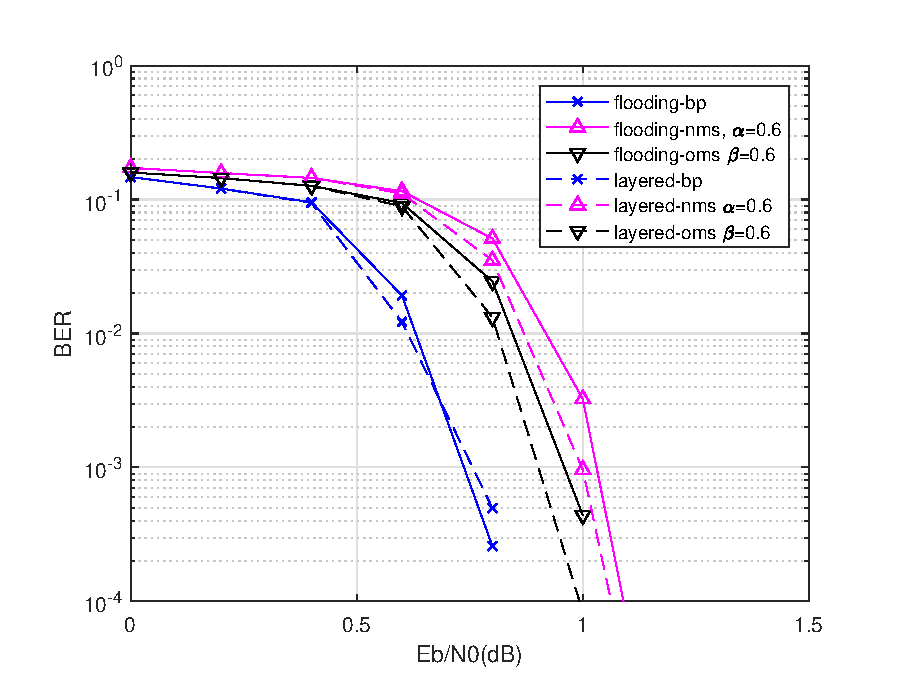
\includegraphics[width = \textwidth]{fig_r12_K8448L.eps}
	\caption{{不同译码算法的误码性能对比($B=8448,R=0.5,I_{max}=50$)}}
\end{figure}
\begin{figure}[H]
	\centering
	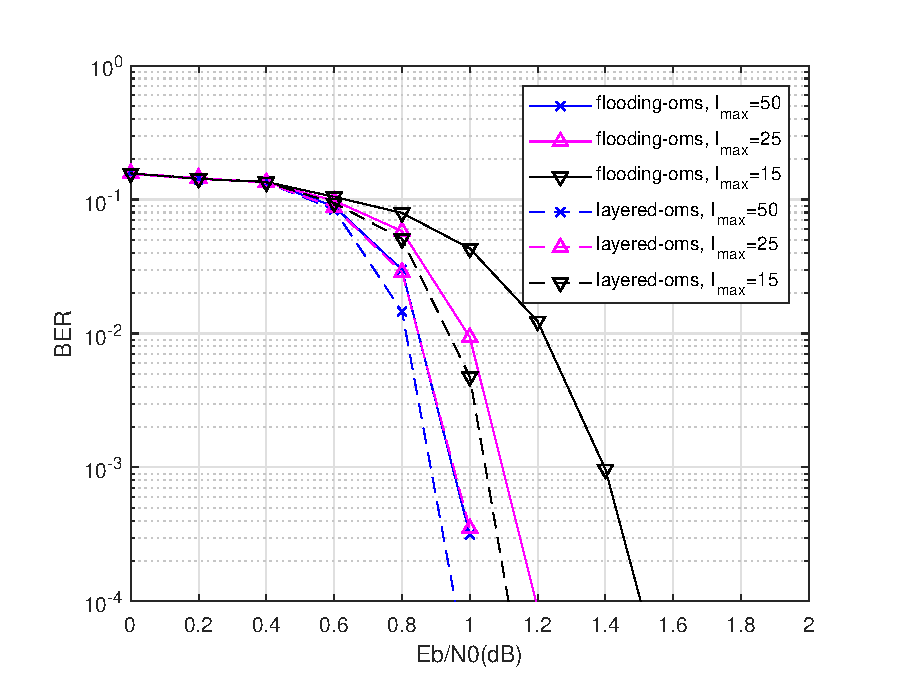
\includegraphics[width = \textwidth]{fig_r12_K8448LImax.eps}
	\caption{{不同译码算法的误码性能对比($B=8448,R=0.5,\beta=0.6$)}}
\end{figure}

%===========第二节=================
% \section{实现LDPC编译码的mex函数编写}



%===========第三节=================
% \section{测试LDPC速率匹配模块}


%===========第四节=================
% \section{仍存在问题}


%===========下周计划=================
\section{下阶段计划}
1. 将message数据类型改为int\_8\\
2. 尝试SIMD改写

\end{document}
%%%%%%%%%%%%%%%%%%%%%%%这是正文部分的结束%%%%%%%%%%%%